\ifx\ISMAIN\undefined
    \documentclass{AsignaturaResumen}
    \SetTitulo{Fenómenos de transporte}
    \setabbreviationstyle[acronym]{long-short}
\makeglossaries

    % Glosario

\newglossaryentry{polimorfismo}{
    name={Polimorfismo},
    description={Existencia de dos o más variantes (alelos) de una secuencia de ADN en una población}
}
\newglossaryentry{locus}{
    name={Locus},description={Posición que ocupa un gen en el cromosoma}}
\newglossaryentry{amplicones}{
    name={Amplicones},
    description={Secuencias de ADN producidas por la amplificación de la hebra original en una \acrshort{pcr}. Se identifican como las bandas de una electroforesis en gel}
}
\newglossaryentry{sucesion microbiana}{
    name={Sucesión microbiana},
    description={Evento donde las especies de microorganismos presentes en una muestran son reemplazadas por otras}
}
\newglossaryentry{variante de secuencia}{
    name={Variante de Secuencia de Amplicón},
    description={Amplicón único de un conjunto de secuencias obtenidas en una secuenciación ya corregida}
}
\newglossaryentry{homopolimero}{
    name={Homopolímero},
    description={Secuencia repetitiva de nucleótidos (AGTGCGAT\emph{AAAA}TGCAGT, p.e.)}
}

    % Acrónimos

\newacronym{si}{SI}{Sistema Internacional}
\newacronym{iubmb}{IUBMB}{Unión Internacional de Bioquímica y Biología Molecular}

\newacronym{ros}{ROS}{especies reactivas de oxígeno}

\newacronym{pb}{pb}{pares de bases}
\newacronym{kb}{kb}{kilobases}

\newacronym{adn}{ADN}{Ácido desoxirribonucléico}
\newacronym{adnc}{ADNc}{ADN complementario}
\newacronym{dntps}{dNTPs}{desoxirribonucleótidos trifosfato}
\newacronym{ddntps}{ddNTPs}{didesoxinucleótidos}

\newacronym{adnpol}{ADNpol}{ADN polimerasa}

\newacronym{pcr}{PCR}{Reacción en Cadena de la Polimerasa}
\newacronym{rapd}{RAPD}{ADN Polimórfico Amplificado al Azar}
\newacronym{rflp}{RFLP}{Fragmentos de Restricción de Longitud Polimórfica}
\newacronym{dpcr}{dPCR}{PCR digital}
\newacronym{ngs}{NGS}{Secuenciación de Nueva Generación}
\newacronym{smrt}{SMRT}{Secuenciación en Tiempo Real de Molécula Única}

\newacronym{ccs}{CCS}{Lecturas de Consenso Circular}
\newacronym{asv}{ASV}{Variante de Secuencia de Amplicón}

\newacronym{iqi}{IQI}{Índice de Calidad Infaunal}

\newacronym{sds}{SDS}{dodecilsulfato sódico}
\newacronym{dms}{DMS}{dimetilsulfato}
\newacronym{ctab}{CTAB}{bromuro de cetiltrimetilamonio}
    \begin{document}
    \chapter{Presión en fluidos}
\fi

%\section{Ecuaciones para el balance de movimiento}



\section{Presión}\label{sec:presion}

Si se requiere calcular la cantidad de kg totales de un fluido se utiliza:

\begin{equation*}
    kg_{\text{Total}} = h_{2}(m) \cdot A(m^{2}) \cdot \rho(kg/m^{2}) = h_{2} \cdot A \cdot \rho_{g} 
\end{equation*}

Para calcular la fuerza total ($F$) del fluido sobre el área 1 debido unicamente al fluido es:

\begin{equation}
    F = (h_{2} \cdot A \cdot P)(g)
\end{equation}

\begin{equation}
    P = \frac{F}{A} \quad\therefore\quad P = h_{2} \cdot \rho_{g}
\end{equation}

Esta es la presión sobre A\sub{2} debido a la masa del fluido que está encima. Sin embargo, para obtener la presión total (P\sub{2}) sobre A\sub{2}debe añadirse P\sub{0}, que soporta todo el líquido, de tal manera que:

\begin{equation}
    F = h_{2} \cdot \rho_{g} + P_{0}
\end{equation}

Esta ecuación es la expresión fundamental para calcular la presión de un fluido a cualquier profundidad.

Para P\sub{1}:

\begin{equation}
    P_{1} = h_{1} \cdot \rho_{g} + P_{0}
\end{equation}

La diferencia entre los dos puntos es:

\begin{equation}
    P_{2} - P_{1} = (h_{2} \cdot \rho_{g} + P_{0}) - (h_{1} \cdot \rho_{g} + P_{0})
\end{equation}

\resumebox{ejercicio}{Calculo de presión}{\footnotesize
    Un gran tanque de almacenamiento contiene petroleo de una densidad igual a \qty{917}{\kg\per\m\cubed}. El tanque tiene una altura de \qty{3.66}{\m} y está abierto a la atmósfera con una presión de 1atm absoluta en la superficie. El tanque está lleno con petroleo a una profundidad de \qty{3.05}{\m} y contiene tambien \qty{0.61}{\m} de agua en la parte inferior. calcule la presión en pascales a \qty{3.05}{\m} de la superficie y en el fondo del tanque. También calcule la presión manométrica del fondo del tanque.
    \begin{figure}[H]
        \centering
        \resizebox{0.45\linewidth}{!}{\begin{tikzpicture}[
    principal/.style={line width=1pt},
    trasera/.style={dashed, line width=1pt},
    flecha/.style={|-Stealth},
    delimitador/.style={|-|, line width=0.75pt},
    texto/.style={font=\sffamily}
]

\draw[principal] (2.5,-2.5) -- (-2.5,-2.5) -- node[pos=0.4] (esq4) {} (-2.5,2.5) -- (2.5,2.5) -- node[pos=0.6] (esq3) {} (2.5,-2.5);
\draw[principal] (-5,0) -- node[pos=0.4] (esq1) {} (-5,5) -- (0,5);
\draw[principal] (-5,5) -- (-2.5,2.5);
\draw[principal] (-5,0) -- (-2.5,-2.5);
\draw[principal] (2.5,2.5) -- (0,5);

\draw[trasera] (0,5) -- node[pos=0.6] (esq2) {} (0,0) -- (-5,0);
\draw[trasera] (0,0) -- (2.5,-2.5);

\draw[trasera] (esq1) -- (esq2) -- (esq3) -- (esq4) -- (esq1);

\draw[delimitador] (3.5,2.5) -- (3.5,0) node[midway, left=0pt, texto] {h$_{1}$};
\draw[delimitador] (3.5,0) -- (3.5,-2.5) node[midway, left=0pt, texto] {h$_{3}$};
\draw[delimitador] (4.5,2.5) -- (4.5,-2.5) node[midway, left=0pt, texto] {h$_{2}$};


\draw[flecha] (-6,4) node[texto, left=0pt] {A$_{0}$} -- (-3.25,4);
\draw[flecha] (-6,1.25) node[texto, left=0pt] {A$_{1}$} -- (-3.25,1.25);
\draw[flecha] (-6,-0.75) node[texto, left=0pt] {A$_{2}$} -- (-3.25,-0.75);

\draw[flecha] (-0.8,6) -- (-0.8,3.75) node[texto, pos=0.8, right=0pt] {P$_{0}$};
\draw[flecha] (-0.8,3.5) -- (-0.8,0.5) node[texto, pos=0.8, right=0pt] {P$_{1}$};
\draw[flecha] (-0.8,0.25) -- (-0.8,-1.75) node[texto, pos=0.7, right=0pt] {P$_{2}$};
\end{tikzpicture}}
        \rule{\linewidth}{0.5pt}
        \caption{Diagrama del tanque}
    \end{figure}
}


\section{Viscosidad} % Ley de Newton y viscosidad

Cuando un fluido se transporta a través de un canal cerrado se presentan dos tipos de flujo dependiendo de dicho fluido:

\begin{enumerate}
    \item A \emph{velocidades bajas} el fluido tiende a transportarse sin mezclado lateral, y las capas adyacentes se resbalan unas sobre las otras. En este caso no hay corrientes cruzadas perpendiculares a la dirección del flujo, ni tampoco remolinos de fluidos. A este tipo de flujo se le llama \emph{flujo laminar}.
    \item A \emph{velocidades altas} se forman remolinos, lo que conduce a un mezclado lateral. A este tipo de flujo se le llama \emph{flujo turbulento}.
\end{enumerate}

La viscosidad es una propiedad de un fluido que da lugar a fuerzas que se oponen al movimiento relativo de capas adyacentes en el fluido. Para muchos fluidos se ha determinado de forma experimental que la fuerza (F) en Newtons es directamente proporcional a la velocidad $\Delta V_{z}$ en metros sobre segundo (\unit{\m\per\s}). El área en metros cuadrados (\unit{\m\squared}) de la placa usada es inversamente proporcional a la distancia $\Delta y$ en metros (\unit{\m}). Expresada con la ley de viscosidad de Newton, cuando el flujo es laminar:

\begin{equation}
    \frac{F}{A} = -\mu \frac{\Delta V_{z}}{\Delta y}
\end{equation}

Donde $\mu$ es la constante de proporcionalidad llamada viscosidad del fluido en pascales por segundo (\unit{\pascal\s}) o \unit{\kg\per\m\s}. Cuando $\Delta y$ tiende a 0:

\begin{equation}
    \tau_{yz} = -\mu \cdot \frac{dV_{z}}{dy}
\end{equation}

\begin{equation}\footnote{lbf/ft\super{2}}
    \tau_{yz} \ gc = -\mu \cdot \frac{dV_{z}}{dy}
\end{equation}

Las unidades en el \emph{sistema cgs} son \unit{\g\m\per\s}, llamados Poise (P) o Centipoise (cp). 

\resumebox{ejercicio}{Cálculo de esfuerzo cortante}{\footnotesize
    La distancia entre las dos placas es de \qty{0.5}{\cm}. La velocidad de flujo que pasa a través es de \qty{10}{\cm\s}, y el fluido que atraviesa se trata de alcohol etílico a \qty{273}{\K}, cuya viscosidad es de \qty{1.77}{cp}.
    \begin{enumerate}
        \item Calcule el esfuerzo cortante $\tau_{yz}$ y el gradiente de velocidad
        \item Repita en SI
    \end{enumerate}
}

\section{Fluidos newtonianos y no newtonianos}

\marginpar{\begin{minipage}{\marginparwidth}
\begin{figure}[H]
    \centering
    \resizebox{\linewidth}{!}{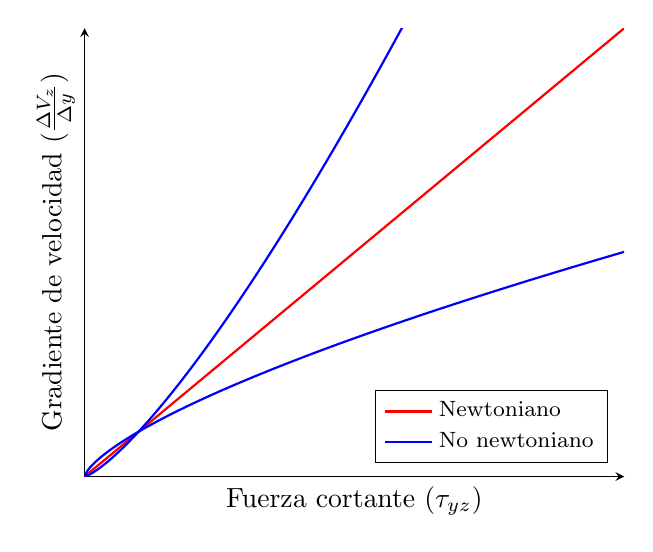
\begin{tikzpicture}
\begin{axis}[
    axis lines = left,
    ticks = none,
    xmin=0, xmax=10,
    ymin=0, ymax=10,
    xlabel = {Fuerza cortante ($\tau_{yz}$)},
    ylabel = {Gradiente de velocidad ($\frac{\Delta V_{z}}{\Delta y}$)},
    domain=0:10, 
    samples=200,
    legend pos = south east,
    legend cell align = left
]
    \addplot[thick, color=red]{x};
    \addlegendentry{\footnotesize Newtoniano}
    \addplot[thick, color=blue]{x^0.7};
    \addplot[thick, color=blue]{x^1.3};
    \addlegendentry{\footnotesize No newtoniano}
\end{axis}
\end{tikzpicture}}
    \rule{\linewidth}{0.5pt}
    \caption{Diferencia entre fluidos newtonianos y no newtonianos}
    \label{fig:grafica_de_tipos_de_fluidos}
\end{figure}
\end{minipage}}

Los fluidos que obedecen la ley de viscosidad e Newton se les llama fluidos newtonianos. En dichos fluidos existe una relación lineal entre el esfuerzo cortante ($\tau_{yz}$) y el gradiente de velocidad ($\frac{\Delta V_{z}}{\Delta y}$), lo cual significa que la velocidad $\mu$ es constante e independiente de la velocidad cortante. En fluidos no newtonianos, la relación entre $\tau_{yz}$ y $\frac{\Delta V_{z}}{\Delta y}$ no es lineal, es decir, $\mu$ no permanece constante, sino que está en función de $\tau_{yz}$.

La viscosidad de los gases, que son fluidos newtonianos, aumenta con la temperatura e independiente de la presión.




% -------------------------------------------------------------------- %

\section{Respuestas de ejercicios}

\resumebox{respuesta}{Calculo de presión}{
\begin{gather*}
    \mathrm{1atm} = \qty{1.01325d5}{\pascal} 
    \quad;\quad
    \unit{\pascal} = \frac{\unit{\kg\m\per\s\squared}}{\unit{\m\squared}} = \unit{\kg\per\m\per\s\squared}
%    \mathrm{P_{n}} = (h_{n} \cdot \rho_{n} \cdot g) + P_{n-1}
    \\\\
    \mathrm{P_{Petroleo}} = \left( \qty{3.05}{\m} \cdot \qty{917}{\kg\per\m\cubed} \cdot \qty{9.81}{\m\per\s\squared} \right) + \qty{1.01325d5}{\kg\per\s\squared\per\m} = \qty{1.2876d5}{\pascal}
    \\
    \mathrm{P_{Agua}} = \left( \qty{0.61}{\m} \cdot \qty{1000}{\kg\per\m\cubed} \cdot \qty{9.81}{\m\per\s\squared} \right) + \qty{1.2876d5}{\kg\per\s\squared\per\m} = \qty{1.3474d5}{\pascal}
    \\
    \mathrm{P_{Fondo (Manométrica)}} = \qty{1.3474d5}{\pascal} - \qty{1.2876d5}{\pascal} = \qty{33415}{\pascal} = \qty{33.415}{\kilo\pascal}
\end{gather*}
}

\resumebox{respuesta}{Cálculo de esfuerzo cortante}{\footnotesize
\begin{enumerate}
\item Calcule el esfuerzo cortante $\tau_{yz}$ y el gradiente de velocidad
\begin{gather*}
    V = \qty{10}{\cm\per\s} 
    \quad;\quad
    \mu = \qty{1.77}{\cp} = \qty{1.777d-3}{\P}
    \quad;\quad 
    y = \qty{0.5}{\cm}
    \\
    \tau_{yz} = \qty{1.77d-2}{\P} \cdot \frac{\qty{10}{\cm\per\s}}{\qty{0.5}{\cm}} = \qty{0.354}{\pascal\s}
    \\
    \frac{\Delta V_{z}}{\Delta y} = \frac{\qty{10}{\cm\per\s}}{\qty{0.5}{\cm}} = \qty{20}{\per\s}
\end{gather*}
\item Repita en SI
\begin{gather*}
    V = \qty{0.1}{\m\per\s} 
    \quad;\quad
    \mu = \qty{1.77d-3}{\pascal\s}
    \quad;\quad
    y = \qty{0.005}{\m}
    \\
    \tau_{yz} = \qty{1.77d-3}{\pascal\s} \cdot \frac{\qty{0.1}{\m\per\s}}{\qty{0.005}{\m}} = \qty{3.54d-2}{\pascal}
%   \\\\
%   \frac{\Delta V_{z}}{\Delta y} = \frac{\qty{10}{\cm\per\s}}{\qty{0.5}{\cm}} = \qty{20}{\per\s}
\end{gather*}
\end{enumerate}
}


\ifx\ISMAIN\undefined
    \end{document}
\fi